\section{Freeze-and-Cut method}

A fundamental assumption in reducing the computational cost of
\textit{ab initio} evaluations is that correlative effects are usually local,
given the nature of the studied phenomena.
For this reason, the molecular framework not involved in chemical or
physical phenomena is an ideal candidate to be frozen at a lower level of
theory, like for example SCF, after the creation of the localized guess.
This strategy has already proved its efficiency in reducing the computational
cost \cite{jms_theo-681-203-2004}, but has no influence on the basis set
size, only the number of molecular orbitals. This is a particularly
severe limitation for MRCI methods, which require a two-electron AO/MO
integral transformation for all correlated orbitals.  This step grows as
$N_{\mbox{\tiny AO}}^4 N_{\mbox{\tiny MO}}$, where $N_{\mbox{\tiny AO}}$ is the number of
Atomic Orbitals (AO) and $N_{\mbox{\tiny MO}}$ is the number of Molecular
Orbitals (MO). If no freezing is performed on the molecular orbitals, the
transformation grows as $N^5$. Freezing a part of the orbital set a
rectangular transformation is performed and the computational
weight is reduced, but the quartic dependence on $N_{\mbox{\tiny AO}}$ still
limits calculations on large AO spaces. This problem must be managed in
order to perform calculations with a reduced dependency of the basis set.

A possible strategy is to cut out the molecular framework that is not
essential for the description of the phenomenon under study.  In other
words, \textit{all the atoms whose AOs are not fundamental in the description
of the non-frozen MOs are eliminated}. The subsequent CASSCF optimization is
performed in the preserved molecular framework only, \textit{under the
effect of the eliminated nuclei and electrons as provided by the freeze}.
This effect takes into account sterical interaction and charge effects
provided by the frozen framework internally (within itself) and externally
(onto the non-frozen framework), given that the AO/MO transformation of the
integrals retains information about the frozen framework.

Moreover, once the CASSCF optimization has been performed, the method
leaves freedom for application of higher levels of theory, still preserving
the effects of the frozen molecular framework at a lower level of theory.

\subsection*{Computational procedure}

The procedure starts with the creation of a set of SCF delocalized orbitals,
which is subsequently localized to obtain a localized SCF set. The resulting
localized orbitals, each one mainly described on a reduced set of atomic functions, are
selected for the freezing step. The remaining unfrozen orbitals are then
projected onto a reduced AO space, setting to zero the coefficients on
those AOs that are not essential for the expression of the orbitals.

\begin{figure}[ht]
\begin{center}
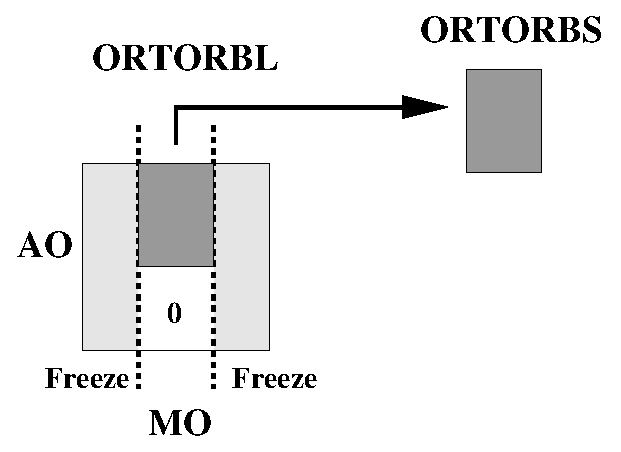
\includegraphics[width=7cm,keepaspectratio]{02_localization/images/matrix.eps}
\caption{\footnotesize A visual representation of large (ORTORBL) and small (ORTORBS)
molecular orbitals matrices. Localized orbitals are first classified as frozen or
non-frozen. The non-frozen orbitals are supposed to have negligible
coefficients on distant atoms. These coefficients are strictly set to
zero by the cut procedure, and a localized optimization is performed in the
obtained AO/MO subspace. }
\label{fig:matrix}
\end{center}
\end{figure}



This procedure leads to two different orbital matrixes. The first one
has the dimension of the original AO basis set, but with some of
the coefficients of non-frozen orbitals set to zero. The second one is
the submatrix of coefficients that belong to unfrozen orbitals
(see Fig. \ref{fig:matrix}).  The latter has a reduced dimension, and
corresponds to the effective space on which the optimization procedure will
be performed.

The orbitals from the two matrixes are no longer orthogonal, and a
hierarchical orthonormalization is performed on the large matrix (non-frozen
orbitals first, then frozen orbitals against the non-frozen ones) and on the
small matrix, to obtain two sets of orbitals, named ORTORBL and ORTORBS
respectively.  An AO/MO integral transformation is performed at each
iteration from the improved orbitals. One-electron MO integrals are provided
by the full dimensional orbital structure, while two-electron MO integrals
are evaluated only on the reduced set described by ORTORBS. 

This procedure results in a spatial confinement of the non-frozen orbitals,
improving the ORTORBS orbitals only inside this reduced AO space. These MOs
have strictly zero coefficients on any AO belonging to the eliminated
region.  For this reason, the method is affected by the truncation of
orthogonalization tails for large basis sets, or in the case of highly
delocalized systems. In general this truncation affects the absolute
energies, with very little effect on the energy differences.

The computational chain is built to interface \molcas 5.4 \cite{molcas-site}, with
a set of small home-developed softwares and bash scripting in GNU/Linux
\cite{gnu-linux-site} environment to provide the complete deployment of this
technique.

A scheme for the method is depicted in Fig. \ref{fig:logical-scheme}.
The scheme focuses on the results (depicted as boxes) obtained through processing steps
(depicted as arrow lines). Thick arrows represent processes that involves evaluation or
use of integrals on the complete system and so represent still a bottleneck
in this technique. Improvements are planned to skip this evaluation, by making
use of a direct SCF procedure.
The formalism can be subdivided into two logical steps:
\begin{itemize}
\item creation of the localized guess (upper part of the scheme)
\item iterative optimization of the localized guess (lower part, enclosed
into dashed frame)
\end{itemize}
The upper part of the scheme can also be subdivided in two independent
calculations: the large calculation, performed on the complete molecular
geometry (left side of Fig. \ref{fig:logical-scheme}) and the small calculation,
performed only on the geometry resulting after the cut operation (truncated
system, right side of Fig. \ref{fig:logical-scheme}).  The localized guess
is obtained through the following strategy:
\begin{itemize}
\item evaluation of the AO integrals on the large system, by using standard
software components from the \molcas 5.4 package
\item calculation of delocalized SCF orbitals
\item creation of a localized guess that describes the bonds or the groups we are
interested in
\item projection of the localized guess onto the SCF delocalized orbitals
\end{itemize}

\begin{figure}[h!]
\begin{center}
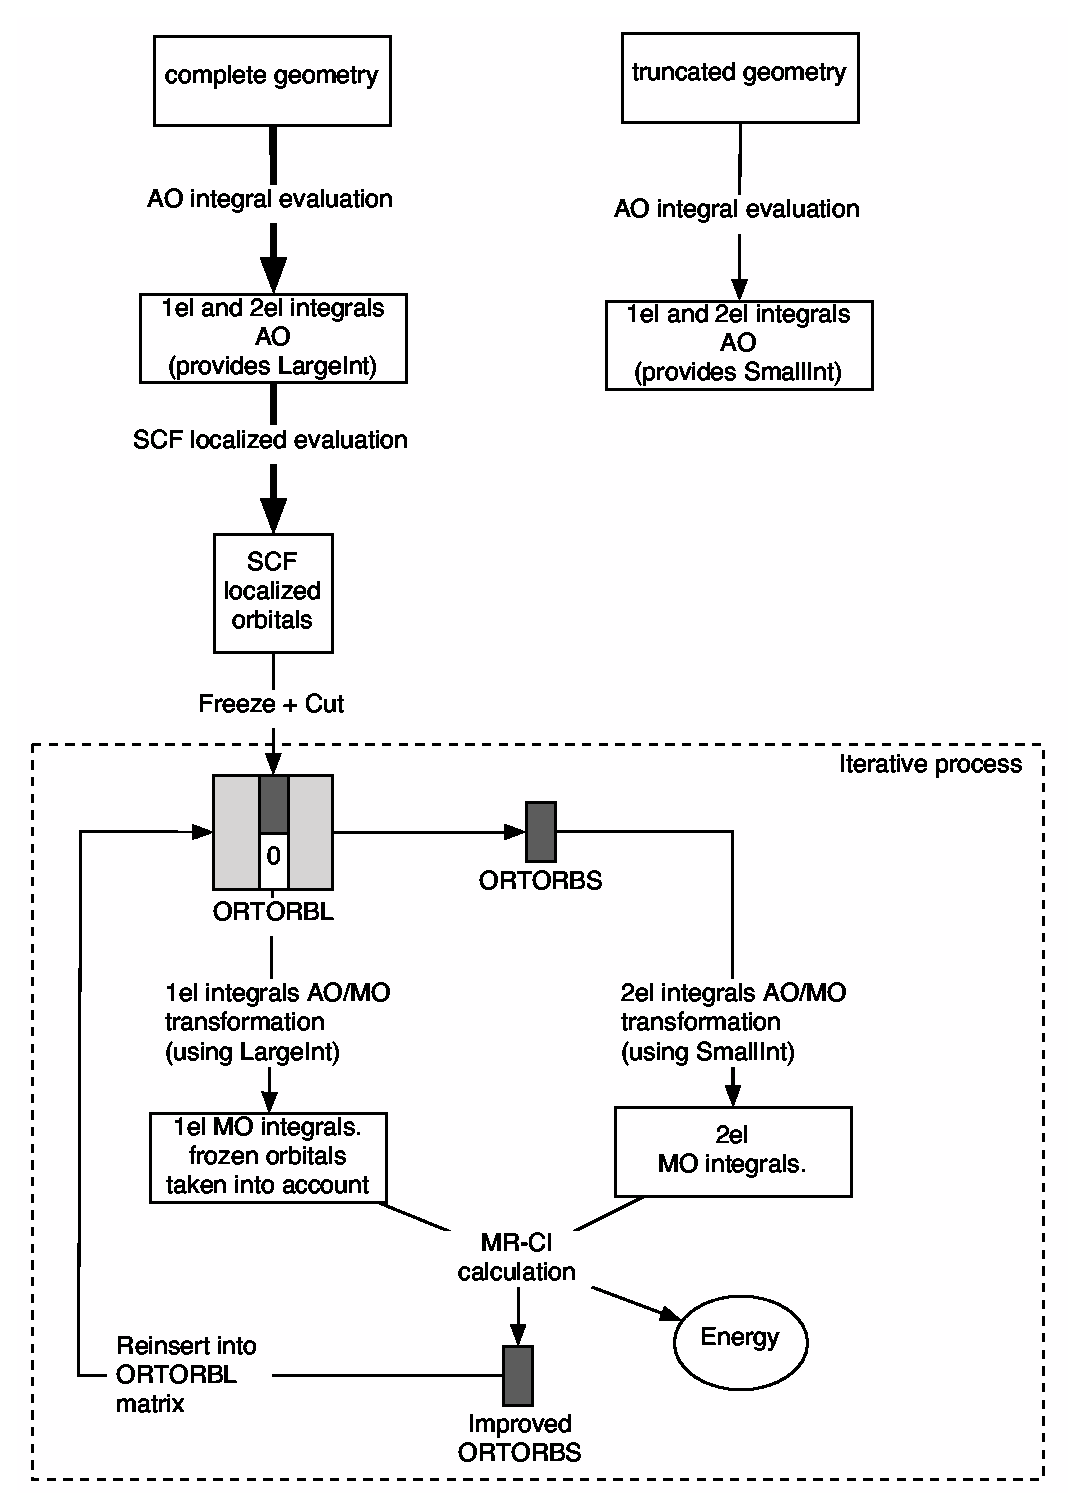
\includegraphics[width=13cm,keepaspectratio]{02_localization/images/logical-scheme-gimped.eps}
\caption{\footnotesize Logical steps (arrows) and obtained entities (boxes) for the
presented procedure. Thick lines denote steps that still depend on two
electron AO integrals on the complete geometry of the system
} \label{fig:logical-scheme}
\end{center}
\end{figure}


These steps describe in more detail the process labeled 
as ``SCF localized evaluation'' in Fig.~\ref{fig:logical-scheme}. The result
is a set of orthogonal localized SCF orbitals.

Thanks to the localization procedure, each localized SCF orbital is mainly
described on a reduced set of atomic basis functions. These orbitals can now
be tagged on two degrees of freedom: the freezing selection of certain
localized SCF orbitals, and the cut of a set of atomic basis functions for
the non-frozen orbitals. The latter is realized by setting to zero the
coefficients that express the non-frozen orbitals on the cut atomic basis
set. This operation effectively projects the non-frozen MO in a reduced
atomic basis space, and the approximation is good as long as the target
coefficients are already close to zero due to the localization.

The large MO matrix (refer to the detailed pictorial representation in
Fig.~\ref{fig:matrix}) holds molecular orbitals that are no longer
orthonormal, although it must be pointed out that the overlap between them
is small. A hierarchical orthonormalization is performed to obtain an
orthonormal set: first the non-frozen orbitals among themselves, then the
frozen occupied orbitals with respect the non-frozen, and finally the frozen
virtual orbitals. Thanks to the hierarchical procedure, the coefficients
that have been set to zero remain unchanged. This is important in order to
keep the non-frozen orbitals inside a smaller AO space.

Finally, a smaller matrix is obtained by extracting the submatrix
of the non-frozen orbitals against the smaller, non-cut atomic set.
The final result of this process are two matrixes, named ORTORBL and
ORTORBS, which hold the molecular orbitals as described, respectively for
the large and the small system (complete system and truncated one).

After an AO/MO integral transformation, the optimization chain is now fed
with two-electron MO integrals (which derive only from orbitals
that are not frozen) and with the modified one-electron integrals that keep
into account the two-electron contribution from the frozen set. 

At each iteration, the procedure works as follows:
\begin{itemize}
\item calculate an improved density matrix using a Super-CI
optimization that preserves orbitals locality. This process is
done only on the restricted subset of non-frozen orbitals, and only on the
available framework of non-cut atoms, leading to an improved set
of orbitals (improved ORTORBS)
\item reinsert the improved orbitals inside the frozen framework, thus creating
an improved ORTORBL large matrix
\item recreate a new set of MO two-electron integrals, transforming the AO integrals
from the truncated system using the improved ORTORBS orbitals
\item recreate a new set of MO one-electron integrals with the improved ORTORBL set
and the complete system
\item iterate until convergence is reached (no change in the energy within a
given level of approximation)
\end{itemize}
